\begin{flushright} {\tiny {\color{gray} basis\_functions\_meaning.tex.tex}} \end{flushright}
%~~~~~~~~~~~~~~~~~~~~~~~~~~~~~~~~~~~~~~~~~~~~~~~~~~~~~~~~~~~~~~~~~~~~~~~~~~~~~~~~~~~~~~~~~~~~~~~~~~


\subsubsection{In one dimension}

Let us consider a 1D domain subdivided in 3 elements. We then consider the four linear basis functions 
attached to each node. On the following sketch these are not depicted on a single element with 
reduced coordinates but instead for the whole domain in the natural coordinate $x$:

\begin{flushright} {\tiny {\color{gray} (tikz\_basisfunctions.tex)}} \end{flushright}
%~~~~~~~~~~~~~~~~~~~~~~~~~~~~~~~~~~~~~~~~~~~~~~~~~~~~~~~~~~~~~~~~~~~~~~~~~~~~~~~~~~~~~~~~~~~~~~~~~~

\begin{center}
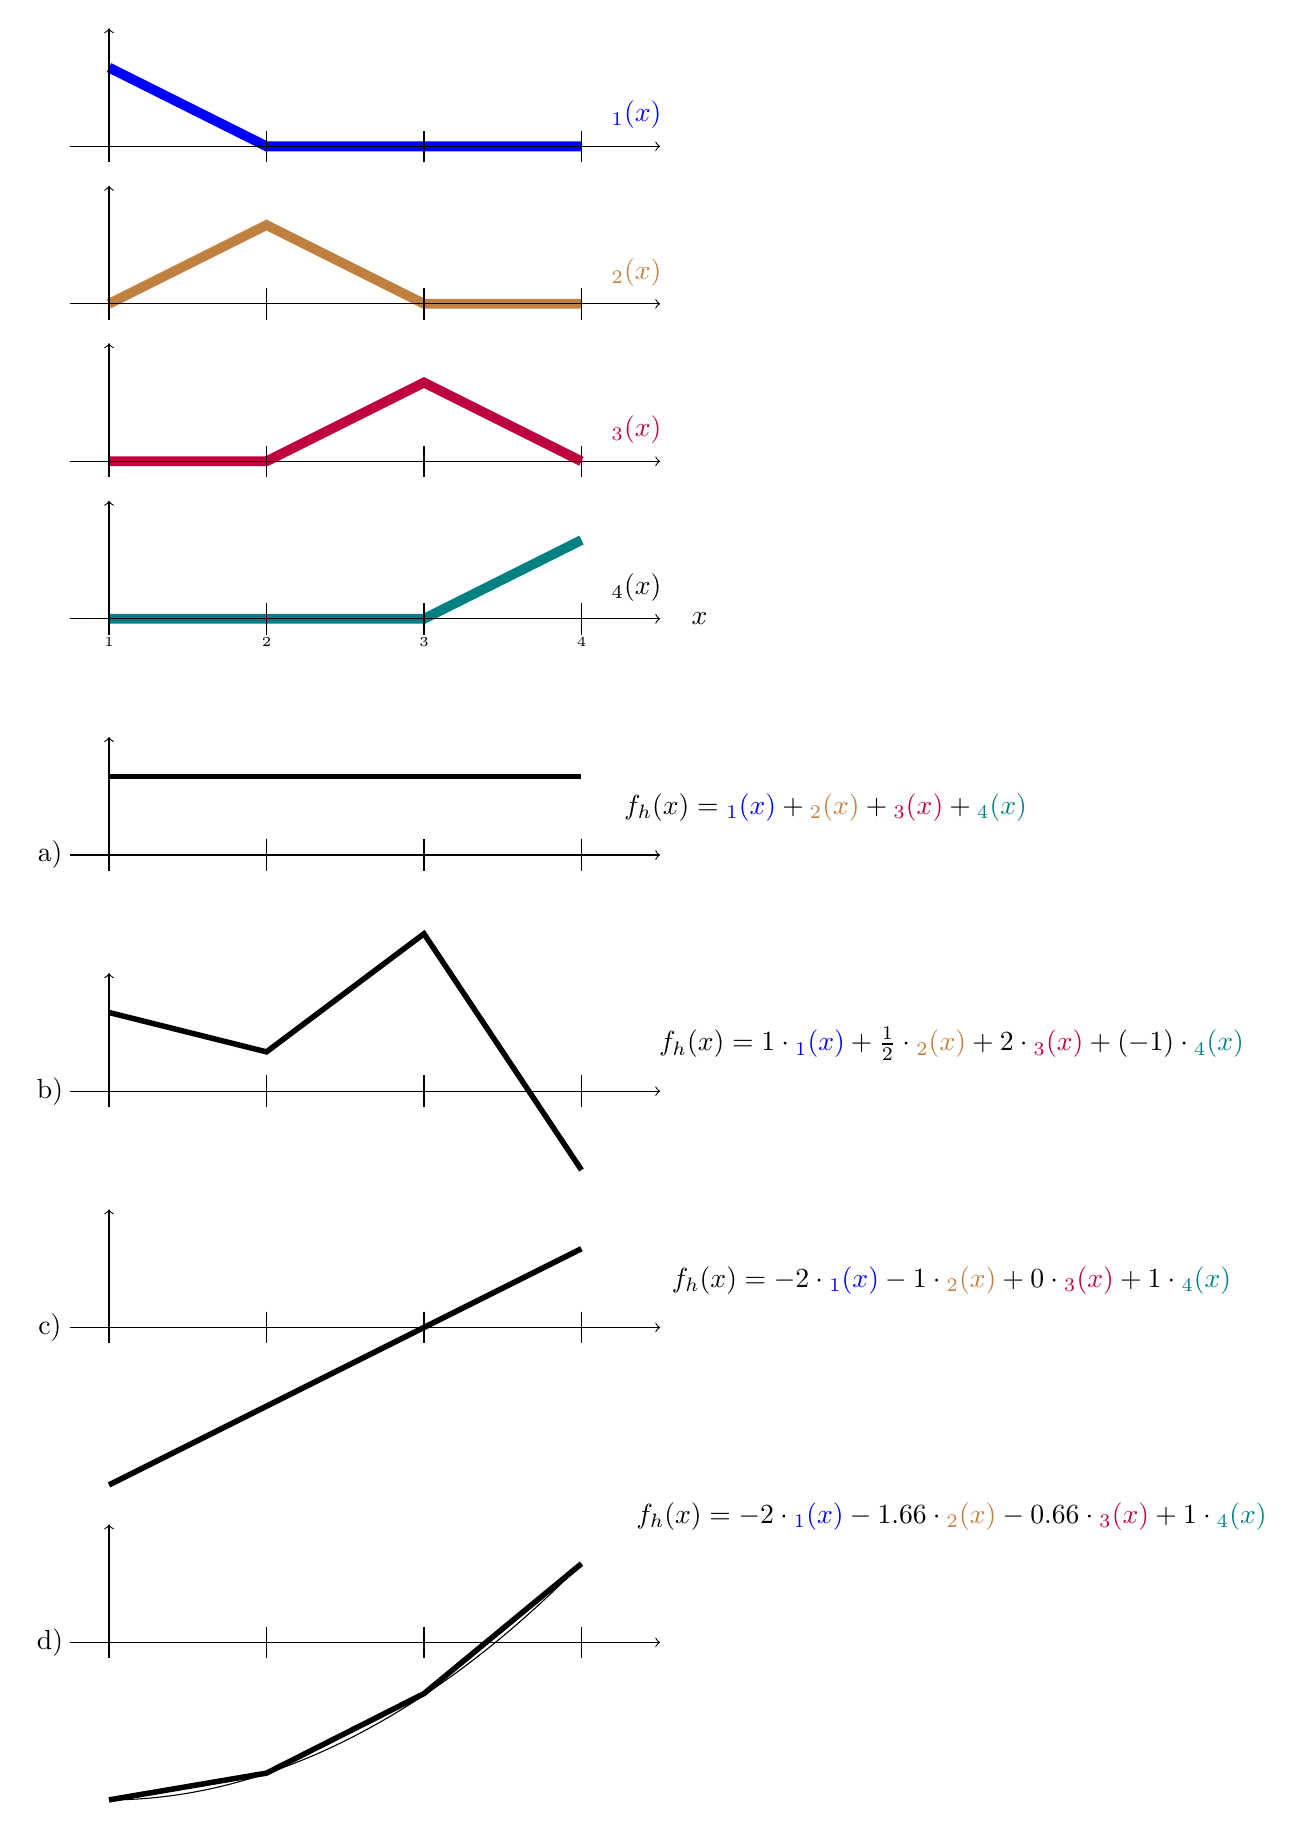
\begin{tikzpicture}
%\draw[step=0.5cm,gray,very thin] (0,-15) grid (15,10); 

%N1
\node[] at (7.7,7.4) {\color{blue}$\bN_1(x)$};
\draw[line width=1.25mm,color=blue] (1,8)--(3,7)--(5,7)--(7,7);
\draw [->] (0.5,7) -- (8,7);
\draw [->] (1,7) -- (1,8.5);
\draw [-] (1,6.8) -- (1,7.2);
\draw [-] (3,6.8) -- (3,7.2);
\draw [-] (5,6.8) -- (5,7.2);
\draw [-] (7,6.8) -- (7,7.2);

%N2
\node[] at (7.7,5.4) {\color{brown} $\bN_2(x)$};
\draw[line width=1.25mm,color=brown] (1,5)--(3,6)--(5,5)--(7,5);
\draw [->] (0.5,5) -- (8,5);
\draw [->] (1,5) -- (1,6.5);
\draw [-] (1,4.8) -- (1,5.2);
\draw [-] (3,4.8) -- (3,5.2);
\draw [-] (5,4.8) -- (5,5.2);
\draw [-] (7,4.8) -- (7,5.2);

%N3
\node[] at (7.7,3.4) {\color{purple}$\bN_3(x)$};
\draw[line width=1.25mm,color=purple] (1,3)--(3,3)--(5,4)--(7,3);
\draw [->] (0.5,3) -- (8,3);
\draw [->] (1,3) -- (1,4.5);
\draw [-] (1,2.8) -- (1,3.2);
\draw [-] (3,2.8) -- (3,3.2);
\draw [-] (5,2.8) -- (5,3.2);
\draw [-] (7,2.8) -- (7,3.2);

%N4
\node[] at (7.7,1.4) {$\bN_4(x)$};
\draw[line width=1.25mm,color=teal] (1,1)--(5,1)--(7,2);
\draw [->] (0.5,1) -- (8,1);
\draw [->] (1,1) -- (1,2.5);
\draw [-] (1,0.8) -- (1,1.2);
\draw [-] (3,0.8) -- (3,1.2);
\draw [-] (5,0.8) -- (5,1.2);
\draw [-] (7,0.8) -- (7,1.2);
\node[] at (8.5,1) {$x$};
\node[] at (1,0.7) {\tiny $1$};
\node[] at (3,0.7) {\tiny $2$};
\node[] at (5,0.7) {\tiny $3$};
\node[] at (7,0.7) {\tiny $4$};

\node[] at (0.25,-2) {a)};
\node[] at (10.1,-1.4) {$f_h(x)={\color{blue}\bN_1(x)}+{\color{brown} \bN_2(x)}
+{\color{purple}\bN_3(x)}+{\color{teal}\bN_4(x)}$};
\draw[line width=0.7mm] (1,-1)--(7,-1);
\draw [->] (0.5,-2) -- (8,-2);
\draw [->] (1,-2) -- (1,-0.5);
\draw [-] (1,-1.8) -- (1,-2.2);
\draw [-] (3,-1.8) -- (3,-2.2);
\draw [-] (5,-1.8) -- (5,-2.2);
\draw [-] (7,-1.8) -- (7,-2.2);

\node[] at (0.25,-5) {b)};
\node[] at (11.7,-4.4) {$f_h(x)=1\cdot {\color{blue}\bN_1(x)}+\frac12\cdot {\color{brown} \bN_2(x)}
+2\cdot {\color{purple}\bN_3(x)}+(-1)\cdot {\color{teal}\bN_4(x)}$};
\draw [->] (0.5,-5) -- (8,-5);
\draw [->] (1,-5) -- (1,-3.5);
\draw [-] (1,-4.8) -- (1,-5.2);
\draw [-] (3,-4.8) -- (3,-5.2);
\draw [-] (5,-4.8) -- (5,-5.2);
\draw [-] (7,-4.8) -- (7,-5.2);
\draw[line width=0.7mm] (1,-4)--(3,-4.5)--(5,-3)--(7,-6);

\node[] at (0.25,-8) {c)};
\node[] at (11.7,-7.4) {$f_h(x)=-2\cdot {\color{blue}\bN_1(x)}-1\cdot {\color{brown} \bN_2(x)}
+0\cdot {\color{purple}\bN_3(x)}+1\cdot {\color{teal}\bN_4(x)}$};
\draw [->] (0.5,-8) -- (8,-8);
\draw [->] (1,-8) -- (1,-6.5);
\draw [-] (1,-7.8) -- (1,-8.2);
\draw [-] (3,-7.8) -- (3,-8.2);
\draw [-] (5,-7.8) -- (5,-8.2);
\draw [-] (7,-7.8) -- (7,-8.2);
\draw[line width=0.7mm] (1,-10)--(3,-9)--(5,-8)--(7,-7);

\node[] at (0.25,-12) {d)};
\draw [->] (0.5,-12) -- (8,-12);
\draw [->] (1,-12) -- (1,-10.5);
\draw [-] (1,-11.8) -- (1,-12.2);
\draw [-] (3,-11.8) -- (3,-12.2);
\draw [-] (5,-11.8) -- (5,-12.2);
\draw [-] (7,-11.8) -- (7,-12.2);
\draw (1,-14) parabola (7,-11);
\draw[line width=0.7mm] (1,-14)--(3,-13.66)--(5,-12.65)--(7,-11);
\node[] at (11.7,-10.4) {$f_h(x)=-2\cdot {\color{blue}\bN_1(x)}-1.66\cdot {\color{brown} \bN_2(x)}
-0.66\cdot {\color{purple}\bN_3(x)}+1\cdot {\color{teal}\bN_4(x)}$};


\end{tikzpicture}
\end{center}


The four cases a,b,c,d are examples of combinations of these basis functions:
\[
f^h(x)=\sum_{i=1}^4 \bN_i(x) f_i
\]
Where $f_i$ are the values associated to the four nodes. 
We assume that the distance $h$ between nodes is 1.

Example a) illustrates the fact that the sum of all basis functions must be strictly equal to one everywhere
in the domain. Failing to do so would mean that the basis functions cannot represent a constant field (see
Section~\ref{ss:q12d}). 

Example b) illustrates a somewhat random combination of the basis functions, yielding a broken line. 

Example c) illustrates the fact that these linear basis functions can exactly represent a
linear function. When $f(x)=x-2$, then $f_1=f(0)=-2$, $f_2=f(1)=-1$, $f_3=f(2)=0$ and $f_4=f(3)=+1$, 
then $f^h(x)$ is exactly $f(x)$ on the domain.

Example d) illustrates the fact that linear basis functions cannot represent a parabola. Smaller and 
smaller elements will do an increasingly better job and will get closer to the curve but a 
systematic error will subsist.  


Note that these drawings are trivial to produce since $\bN_i(x_j)=\delta_{ij}$ by definition, so that 
$f^h(x_j)=f_j$.

%........................................................................
\subsubsection{In two dimensions}



